\documentclass[11pt,a4paper,runningheads]{llncs}
\usepackage[utf8]{inputenc}
\usepackage{amsmath}
\usepackage{amsfonts}
\usepackage{amssymb}
\usepackage{graphicx, svg}
\usepackage{xcolor}
\usepackage[backend=bibtex, style=numeric]{biblatex}
\usepackage{hyperref}
\usepackage{xspace}
\usepackage{tcolorbox}

% code listings
\usepackage{listings}

\definecolor{codegreen}{rgb}{0,0.6,0}
\definecolor{codegray}{rgb}{0.5,0.5,0.5}
\definecolor{codepurple}{rgb}{0.58,0,0.82}
\definecolor{backcolour}{rgb}{0.95,0.95,0.95}

\lstdefinestyle{stolenstyle}{
    backgroundcolor=\color{backcolour},
    commentstyle=\color{codegreen},
    keywordstyle=\color{magenta},
    numberstyle=\tiny\color{codegray},
    stringstyle=\color{codepurple},
    basicstyle=\ttfamily\footnotesize,
    breakatwhitespace=false,
    breaklines=true,
    captionpos=b,
    keepspaces=true,
    numbers=left,
    numbersep=5pt,
    showspaces=false,
    showstringspaces=false,
    showtabs=false,
    tabsize=2
}

\lstset{style=stolenstyle}

\input{llvm}

% ————————————————————————————————— Commands ————————————————————————————————— %

\newcommand{\ie}{\textit{i.e.}\xspace}
\newcommand{\amd}{\textsf{x86\_32}\xspace}
\newcommand{\riscv}{\textsf{RISC-V}\xspace}
\newcommand{\llvm}{\textsf{LLVM}\xspace}
\newcommand{\bpf}{\textsf{BPF}\xspace}
\newcommand{\serval}{Serval\xspace}
\newcommand{\racket}{\textsf{Racket}\xspace}
\newcommand{\rosette}{\textsf{Rosette}\xspace}
\newcommand{\zthree}{\textsf{Z3}\xspace}
\newcommand{\clang}{\textsf{C}\xspace}
\newcommand{\gcc}{\textsf{gcc}\xspace}
\newcommand{\cclang}{\textsf{clang}\xspace}

    % notes
\newcommand{\sankalp}[1]{\textcolor{red}{[Sankalp: #1]}}
\newcommand{\charly}[1]{\textcolor{green}{[Charly: #1]}}
\newcommand{\can}[1]{\textcolor{blue}{[Can: #1]}}

% ———————————————————————————————— Meta-Data ————————————————————————————————— %

\title{--- CS550 Project Report --- \\ Extending symbolic evaluation for automated verification of systems
code with loops in \serval}
%\subtitle{Formal Verification Background Paper Report}
\author{
    % alphabetic by last name
    % Charly Castes \\ \texttt{charly.castes@epfl.ch} \and 
    % Can Cebici\\ \texttt{can.cebici@epfl.ch} \and
    % Sankalp Gambhir \\ \texttt{sankalp.gambhir@epfl.ch}
    Charly Castes \qquad Can Cebeci \qquad Sankalp Gambhir
    \\
    \texttt{\{firstname.lastname\}@epfl.ch}
    }
\institute{
    EPFL
}

\authorrunning{Castes, Cebeci, Gambhir}
\titlerunning{Project --- Loops in \serval}

    % biblatex
\bibliography{biblio}

% ——————————————————————————————— Quick Notes ———————————————————————————————— %

% WARNING: might or might not be useful
%
% - With \serval developers write a system using standard languages and tools, such
%   as C and GCC, as well as a specification using a language called Rosette (a
%   dialect of Racket) to generate a query that can be checked by a SMT solver.
% - Rosette provides a decidable subset of first-order logic.
% - To create a new verifier for a given ISA, it suffice to write an interpreter
%   in Rosette and with the help of the Serval library.
% - Rosette has an helpful feature that allows finding performance bottle-necks,
%   this can be used to identify what causes verification to be slow/hang within
%   the interpreter.
% - An example of performance bottleneck is when the PC becomes symbolic (i.e.
%   after a conditional jump that might result in two different locations),
%   interpretation becomes very expensive compared to a fixed-value PC. Serval
%   provides domain-specific optimization, for instance through the `split-pc`
%   functions which revert the state merging on PC, making it a concrete value
%   instead of a symbolic one.
% - Serval verifies that:
%   1. If the invariants hold on the initial state, they hold for the final
%      (symbolic) state.
%   2. If the invariants hold and the initial state is mapped to the spec initial
%      state (through a user-provided mapping function), then the final symbolic
%      state is mapped to the final symbolic state of the specification through
%      the same function.
% - Systems such as kernel or hypervisors works by responding to events, such as
%   booting or responding to a trap. When reacting to an event, the system is in a
%   well known state, with the exception of some values (such as registers) than
%   can depend on user programs and are therefore represented by a symbolic value.
% - Serval uses `objdump` to read the assembly instructions, but `objdump` is not
%   part of the trusted code base (TCB) as Serval also implements an encoding
%   function that is used to validate that `objdump`'s output can indeed be
%   re-encoded in the exact same binary.
% - Serval represents memory as a set of disjoint blocks, similar to KLEE and
%   ComCert.
% - The paper describes a set of optimizations that should be applied at the
%   interpreter or specification level in section 4.
% - Serval itself is ~1200 LoC, each verifier is around ~1000 LoC (a bit less
%   usually).

% ————————————————————————————————— Document ————————————————————————————————— %

\begin{document}
\maketitle

\noindent
\begin{minipage}{\textwidth}
    Github repository with all files:

    \begin{center}
        \url{https://github.com/sankalpgambhir/cs550-project}
    \end{center}

    Paper reference:
    
    \fullcite{serval}
\end{minipage}

\section{Introduction}

In this project, we extend \serval \cite{serval}, a framework for building
Push-Button Verifiers (PBV) for system software, such as kernels, by performing
symbolic execution on assembly code. The main motivation for PBV is to
drastically reduce the cost of writing proofs, which is often measured in
person-years and whose size can be orders of magnitude the size of the code for
system software \cite{sel4}.

We believe \serval is a good target for further study and extension. Due to its
nature of building portable verifiers, it is applicable to verification of a
wide variety of systems code, whilst reducing the size of involved trusted code
bases. However, the verification itself relies on a simple symbolic execution
model with some optimizations to aid solving. In particular, it naively unfolds
all loops and branches, limiting its application to software with finite
interfaces. In the rest of this report, we discuss an extension to \serval, in
the form of recognition and verification of loop invariants, that significantly
improves the applicability of the tool, without adding significant proof effort.

% \serval improves on previous approaches by (1) completely removing the need for
% writing proofs, and (2) proposing a portable approach for defining fully
% automated verifiers. 
% In the current implementation, these benefits come at the cost of being able to
% verify only programs that produces traces of bounded length, \ie{} programs with
% \textit{finite interfaces}.

% The paper evaluates \serval by building verifiers for \amd{}, \riscv{}, \llvm{},
% and \bpf{} instruction sets.
% These verifiers are then used to verify two previously verified systems
% (CertikOS \cite{certikos} and Komodo \cite{komodo}) and two existing but
% unverified systems (the Keystone monitor \cite{keystone} and the \bpf{}
% compiler).

% In this report we first give some background on push-button verification
% (\S\ref{context}), then give an overview of the \serval verification stack
% (\S\ref{serval}), detail why it is well suited for verifying system software
% (\S\ref{system}), and highlight some of the limitations of the proposed
% approach.

\section{Context and Background}
\label{context}

Current methods for verifying systems software come with high proof effort. Both
the use of interactive theorem provers (e.g. Isabelle/HOL \cite{isabelle}, Coq), and annotation
based auto-active proof systems (Dafny \cite{dafny}) usually require time investments in the
order of person-years. Among the well-known examples, the
proof-to-implementation ratio varies from 4.8:1 (Ironclad \cite{ironclad}) to 20:1 (seL4 \cite{sel4})

\textit{Push-button verification} is an alternative approach that reduces the proof
burden at the cost of generalizability. 
In order to be applicable, it requires the target software to be
\textit{finite}, i.e., free of unbounded loops. 
Push-button verifiers compile such software into a formula through symbolic
evaluation, and then invoke a solver to verify desired properties. 
While the finiteness limitation is restrictive, considering automated verification as a
first-class goal in system design can enable the construction of practical,
large-scale, push-button verified systems.
% Moreover, certain classes of systems software, for instance security monitors,
% naturally lend themselves well to finite designs and implementations.

% Writing push-button verifiers is cumbersome and the verifiers are not reusable.
% A push-button verifier often needs a symbolic evaluator to be written for the
% specific system to be verified, as it needs to capture the relevant subset of
% the target language. In order to make symbolic evaluation scale to more complex
% software, the symbolic evaluator has to minimize path explosion, which requires
% domain-specific optimizations. The need to repeat this process per target system
% not only increases the required development effort but also makes the verified
% system less reliable, as the symbolic evaluator is inevitably trusted.

\section{\serval Verification Stack} 
\label{serval}

\serval is a framework for building specialized verifiers operating at the
instruction set level. Developers define a standard interpreter for a given
instruction set which \serval then ``lifts'' into a verifier. By virtue of
dynamic typing, a lifted interpreter can be readily used with both concrete and
symbolic values.

The framework itself is written \racket{}, a dynamically
typed language, and builds on top of the \rosette{} symbolic evaluation library.
%
\rosette{} is a solver-aided programming language, which extends Racket to provide
constructs for verification in a decidable fragment of first-order logic: with
booleans, bit-vectors, uninterpreted functions, and quantifiers over finite
domains.
%


To verify systems software with \serval, the developer needs to provide a raw
instruction stream (obtained using standard system code and tools such as \clang{} and
\gcc), and a specification.
%
The specification consists of four definitions: an abstract specification state $s$, a functional
specification corresponding to the intended behavior $f_{spec}$, an abstraction
function $AF$ that maps a concrete state $c$ to an abstract specification state, and a
representation invariant $RI$ that must hold before and after the execution of every system service.
\serval then checks that the concrete implementation is a \textit{refinement} of
the abstract specification.

To do so, \serval computes the symbolic states reached by running the
implementation on concrete state $c$ and by running the functional specification
on equivalent abstract state $s$, denoted $f_{impl}(c)$ and $f_{spec}(s)$
respectively. Then, it checks that the representation invariant is maintained:

$$
RI(c) \Rightarrow RI(f_{impl}(c))
$$

and that the implementation and the specification move in lock-step:

$$
 (RI(c) \land AF(c) = s) \Rightarrow AF(f_{impl}(c)) = f_{spec}(s)
$$


% \section{Temp: Why is Serval/Rosette?}
% - serval modularizes the symbolic execution
% - allows for optimizations based on the memory model under consideration
% - rosette's extensive symbolic framework allows for easy and natural expression of theorems

Instead of implementing its own symbolic execution framework, \serval relies on
the extensive framework provided by \rosette, from which it inherits several
powerful features, such as its \emph{symbolic profiling}, which identifies
bottlenecks in execution and verification to assist iterative code and
specification development.

Writing a specification requires a deep embedding of the system state in
\racket/\rosette. However, as opposed to high-level functional verification,
\serval pushes the embedding to be performed on the level of the system
architecture, so the modelling is inherently finitely-structured
(register-model), which makes it more easily amenable to automated verification. 

The \serval implementation models its memory within \racket as well, which allow
for optimizations for the symbolic execution at runtime. In particular, \serval
also implements optimizations possibly unsound for symbolic execution by adding
extra verification conditions to account for issues like overflow in the
specific program path. In essence, this implements conditional rewrites, and
allows for significant reduction in path explosion, by assisting state merging
during the execution. 

Writing an interpreter on top of \serval makes these optimizations uniformly
available, alongside \rosette's wide array of solver-aided debugging and
synthesizing features. Based on the generation of unsat-cores from solvers,
\rosette can identify problematic sections (termed \emph{localizing}
\cite{rosette}) of functions and even synthesize equivalent functions for
reduction or function patches for debugging.

While \rosette's framework would allow for inserting a rich array of
intermediate conditions to assist solving akin to Stainless \cite{stainless},
\serval bypasses this in favor of automation, limiting it to verification of
finite interfaces. We believe there is a different balance that can be struck
whilst maintaining a similar level of specification from the developers, but
extend \serval to then support a much larger class of systems.

Given this extension, it may be interesting to explore ideas such as termination
checking and reachability for black-box binaries.

% Todo: execution model i.e. trap handlers

\section{Verifying Systems Software}
\label{system}

Serval targets the verification of system code, such as OS kernels and security
monitors.
This imposes constraints on the choice of implementation language, size of the
trusted code base and requires special considerations regarding the control flow
of the program.

\subsection{Assembly-Level Verification}

System software are subject to strict requirements regarding both performance
and security.

From a performance point of view, system software must of course execute fast,
but more importantly with predictable latency.
In particular, higher level languages with automatic garbage collections can not
be used due to the GC pauses.
Regarding security, system software aim to minimize the trusted code base (TCB).
For bare metal kernels or security monitors the TCB usually consists in the
compiler and verification toolchains.

To address both issues, Serval takes the stance of verifying assembly code
directly.
This makes Serval compatible with existing toolchain such as \gcc{} or \cclang{}
without including the whole compiler in the TCB, effectively preventing compiler
backdoor attacks \cite{trustingtrust}.
In practice, the TCB of a program verified using Serval consists in Serval
itself (1200 LoC), the interpreter (usually around 1000 LoC), \rosette{} and
\racket{}.

\subsection{Execution Model}

The control flow of privileged system software usually differs from those of
userspace programs.
The life-cycles of a kernel starts with an initial boot sequence followed to
a context-switch to isolated user-space programs.
At that point, the system is fully initialized and will regain control only
through well defined entry points in reaction to user requests (\ie system
calls), exceptions, or hardware interrupts.
The different handlers for those events are usually short-lived, and in the case
of security monitors mostly perform checks before granting access to a resource.
Those properties make handler functions good candidate for push-button
verification, because they often only allow for a finite number of execution
traces that can be exhaustively checked using symbolic execution.

\section{Limitations}

Serval trusts the verification toolchain, the specification library, and hardware.
As mentioned above, Serval treats the interpreter used to construct a symbolic
evaluator as a specification for the target instruction set, and thus trusts it.
Any toolchain that may be used to compile source code to the target instruction
set, however, is not trusted.

Serval can not reason about concurrent code, it assumes a single-core,
single-threaded environment. 
Similarly to prior work, it also assumes that interrupts are disabled while
executing security monitor code.

Lastly, Serval sacrifices generality in favor of proof automation. 
Adopting the approach of push-button verification, it requires systems to be
finite and it can not deal with implementation code that includes
potentially unbounded loops. It is based on naive symbolic evaluation and it
does not make use of state-of-the art verification techniques that allow other
verification frameworks to automatically infer measures or loop invariants.

% extension, do ont treat loops transparently
\section{Extension: Inductive Verification}

We implement our extension within the Racket based LLVM Intermediate
Representation (IR) interpreter supplied with Serval's distribution. The choice
is justified in \autoref{subsec:llvmir}, along with other possible options for
generalisation.

In a nutshell, we identify loops in (unoptimized) LLVM IR and insert a special
instruction to identify a looping edge. We extend the interpreter to process
this instruction as checking the loop invariant and then pruning the branch. The
process of identification and the transformation are described further in
\autoref{subsec:loopident} and \ref{subsec:looptransform} respectively.

\subsection{Loop identification}
\label{subsec:loopident}

To deal with loops, we must first identify them. This turns out to not be a
straight-forward task when dealing with IR and assembly code. Take, for example,
the following two excerpts of IR:

\begin{lstlisting}[language=llvm]
 %i.05 = phi i32 [ 0, %entry ], [ %inc1, %for.body ]
 %inc1 = add nuw nsw i32 %i.05, 1, !dbg !949
 %exitcond.not = icmp eq i32 %inc1, 10, !dbg !953

 br i1 %exitcond.not, label %for.cond.cleanup, label %for.body, !dbg !947, !llvm.loop !954
\end{lstlisting}

\begin{lstlisting}[language=llvm]
 %3 = load i32, ptr %j, align 4, !dbg !924
 %cmp2 = icmp sge i32 %3, 10, !dbg !926
 br i1 %cmp2, label %if.then, label %if.else, !dbg !927
 
 store i32 -1, ptr %retval, align 4, !dbg !928
 br label %return, !dbg !928
\end{lstlisting}

It is easy in this case to spot the labels for \texttt{for} and \texttt{if} if
one looks carefully, but from the instructions themselves, it is not immediate
what the structures represent, which are a for-condition and an if-entry
respectively. Thus, in this case it becomes imperative to order and track the
branch locations to differentate conditionals from loops. This forms the
fundamental idea of loop identification: 

\paragraph{Control flow graph cycle detection ---}
%
To track branch points, we begin with a standard method, of collapsing code
blocks (which as blocks are either branch points or branch targets) and
generating from them a control-flow graph (CFG). A loop is now simply
represented as a graph cycle. The identification of blocks and construction of
the CFG are facilitated by the LLVM library \cite{clang}. While this method
works well by itself, during testing, we want to focus attention to certain
loops that carry invariants. To achieve this, we utilize the already present
information about block labels.

\paragraph{Annotation assisted cycle detection ---}
%
In our implementation, we use a simple extension of the CFG cycle detection
method, wherein we raise a flag and perform checks only when within a
\texttt{for.cond} or \texttt{for.body} block to limit the cycle detection
needlessly exploring the entire CFG, as well as to draw focus on loops we intend
to verify.

\subsection{Loop tranformation}
\label{subsec:looptransform}
%
Once a loop has been identified, we transform it to be read by our extended
interpreter and subsequently verified. This is diagrammatically presented in
\autoref{fig:origloop} and \ref{fig:modloop}.

% formal transformation
\begin{figure}[!ht]
    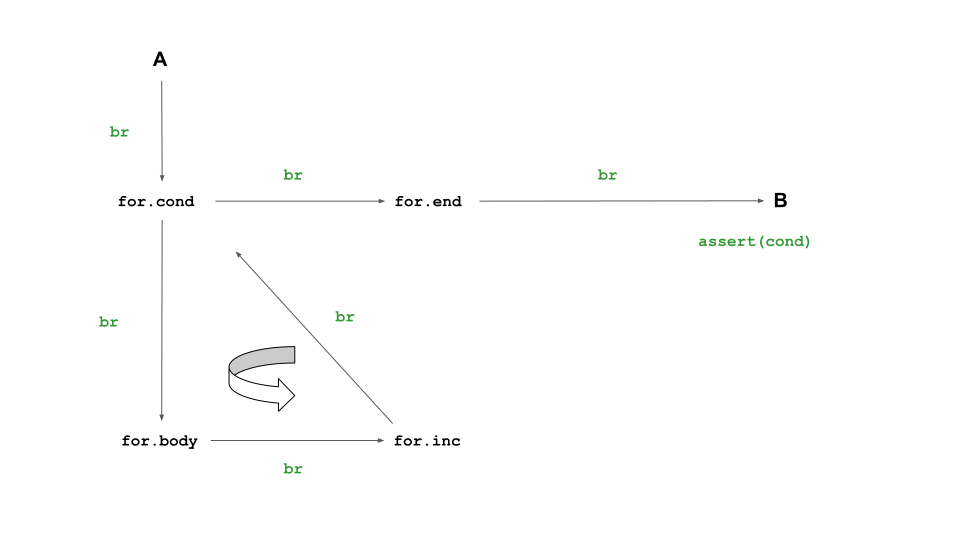
\includegraphics[width=\textwidth]{fig/original_loop.pdf}
    \caption[Loop CFG]{Control flow graph of a simple loop.}
    \label{fig:origloop}
    
    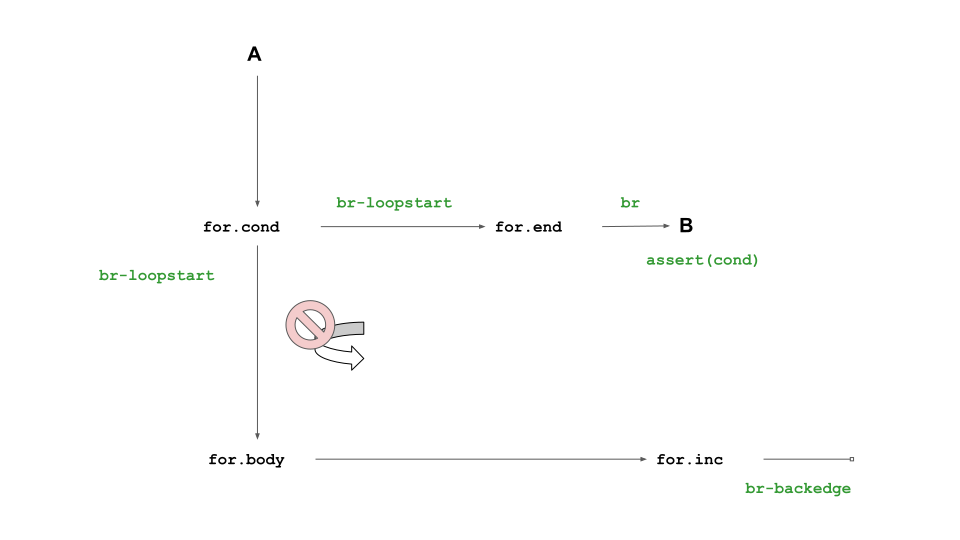
\includegraphics[width=\textwidth]{fig/modified_loop.pdf}
    \caption[Changed CFG]{Modified control flow graph to incorporate invariant verification.}
    \label{fig:modloop}
\end{figure}

The transformation involves two major changes:

\begin{enumerate}
    \item \texttt{br-loopstart} --- all outgoing branches (\texttt{br}) from the
    for-condition block are relabelled as loop-start instructions
    (\texttt{br-loopstart}). When interpreted, these append the loop invariant
    to the current context for verification.
    \item \texttt{br-backedge} --- the looping branch from the for-increment
    block is relabelled as a backedge (\texttt{br-backedge}). Contrary to the
    name, this instruction is not in fact interpreted as a branch point. This
    breaks the loop structure and bounds the verification by pruning the loop
    branch. Instead, it expresses a signal to construct an inductive proof and
    complete verification of the loop (\autoref{subsec:inductivever}).
\end{enumerate}

\subsection{Invariant verification}
\label{subsec:inductivever}

To verify a transformed loop, we interpret the branch instructions to perform
`inductive symbolic execution'. This approach which leverages loop invariants to
avoid loop unrolling-caused path explosion. The loop invariant is a formula over
the variables within the program's execution state that holds at the beginning
of every iteration of a given loop. Instead of unrolling a loop, inductive
symbolic execution uses the loop invariant to safely overestimate the set of
program states that are reachable at the start of the loop.

When a loop is encountered, a inductive symbolic executor checks that the path
condition implies the loop invariant, which constitutes the base case for an
inductive proof that the loop invariant is correct. To prove the inductive step,
the executor generalizes the symbolic memory to capture the state of the system
after an arbitrary number of iterations of the loop: it replaces all variables
that are potentially modified by the loop with fresh symbolic variables and
assumes the loop invariant by adding it to the path condition. Then, it resumes
symbolic execution as usual, pruning the branch that loops back.

Over looping branches, it checks whether the path condition implies the loop
invariant, proving the inductive step for that path. This concludes symbolic
execution for that path, and so the loop is never unrolled. Paths that exit the
loop readily assume the loop invariant, as the generalization step adds the
invariant to the path condition. The invariant is useful if this assumption
suffices to prove the desired properties about the rest of the program.

Our extension does \emph{not} directly modify the symbolic executor built into
Rosette. Instead, we facilitate inductive symbolic execution within our
extension to the LLVM interpreter such that it reuses Rosette's context, and
then stitches the resulting formulas together equivalently to what an inductive
symbolic executor would do.

Formally, this corresponds to the standard representation of a loop in terms of
its invariant. Given formulas \(C(\{x_i\})\) representing the loop condition and
\(L(\{x_i\})\) representing the invariant, with \(\{x_i\}\) standing in for
variables representing the loop state, an initial state given by the assignment
to the variables as \(\{x_i^0\}\), and a function \(f(\{x_i\})\) representing
the loop body, mapping a state at the start of the body to one after its
execution, the loop verification condition is given by

\begin{equation}
    \texttt{loop-vc} = L(\{x_i^0\}) \land \left[~\forall \{x_i\}.~ C(\{x_i\}) \implies L(f(\{x_i\}))~\right]
\end{equation}

\begin{figure}[!ht]
    \begin{lstlisting}[language=C++]
 bool loop_inv = i >= 0 & i <= 10;
 
 for(int i = 0; i < 10; i++){
     j++;
 }
    \end{lstlisting}
    \caption[C++ Loop]{A simple for-loop in C++.}
    \label{fig:cpploop}

    \begin{lstlisting}[language=llvm]
 entry:
     %i = alloca i32, align 4
     %loop_inv = alloca i32, align 4
     ...
     store i32 %and, i32* %loop_inv, align 4
     br label %for.cond
 
 for.cond:
     ...
     br i1 %cmp, label %for.body, label %for.end, !dbg !68
 
 for.body:
     ...
     br label %for.inc, !dbg !71
 
 for.inc:
     ...
     br label %for.cond, !dbg !73, !llvm.loop !74
    \end{lstlisting}
    \caption[LLVM Loop]{A simple for-loop compiled to LLVM IR with labelled sections (\textsf{-O0}).}
    \label{fig:llvmloop}
\end{figure}

\subsection{Choice of LLVM IR and Generalisation}
\label{subsec:llvmir}

The choice of LLVM IR for this extension is motivated by many features we gain
with LLVM, largely in the interest of time:

\begin{itemize}
    \item LLVM's C++ library offers extensive methods to conveniently read and
    process IR. In fact, this is already in use within Serval to process IR and
    translate it to executable Racket code.
    
    \item The \cclang compiler \cite{clang} which outputs the IR from an input
    program also prints readable annotations to identify loops (see
    \autoref{fig:llvmloop}), which assisted the initial development and
    subsequent automation of loop transformation greatly.
\end{itemize}

However, since this transformation requires an extension of the interpreter to
sidestep loops, \emph{it does break the soundness of the execution}. The \racket
version of the code is no longer simply executable by calling the interpreter as
before. While this may not be a breaking point in most scenarios, it is not a
necessary tradeoff to make for this extension.

For generalisation, and to maintain the soundness of the interpreter, the
backedge detection can be performed within \rosette directly. This would make
the transformation an internal operation to the verifier, and crucially,
disjoint from the interpreter. This would also allow for effortless
generalisation to different languages without modification to the interpreters,
or the use of other language specific libraries. However, this would be a much
larger project requiring a deeper survey of the \rosette architecture and would
come with a significant implementation effort attached.

\section{Conclusion}

The \serval framework proposes an interesting solution to the push-button
verification of system software, but also suffers from severe limitations. We
extended \serval with identification and verification of loop invariants by
appending to the interpreter. Our extension was limited to the LLVM interpreter
within \serval, but the techniques form a base for a possible generalised
extension to the \serval and \rosette pipeline. 

% single core, interrupt disables, finite interface

% \section{Preliminaries}
% State the technical details that are necessary to understand the paper. It is
% generally a collection of definitions, concepts and notations with potentially a
% few preliminary results. It can be, for example the mathematical framework in
% which the topic of your paper is expressed. In particular, fix the notation you
% will be using for your review.
%
% \section{Body}
% Explain the paper, in your own words. Don't go into as many details as the
% original text, but the person reading your review should have a general
% understanding of the paper's results and how those results can be obtained. The
% structure and content of this section of course heavily depends on the paper
% itself. Don't hesitate to split it in multiple sections or subsections, for
% example:
% \subsection{An algorithm for whatever problem we try to solve}
% If your paper contains theorems, sketch the proofs of important theorems.
%
% \subsection{Benchmarks}
% If it contains benchmarks, show the key scores or results.
%
% You can follow the structure of the paper you're reviewing, but write with your
% own words.
%
% \section{Conclusion}
% Recall  briefly what the paper achieves, and how it is new. Express your
% critical skil on the paper and explain what you think are the strong and weak
% points of the paper. Also tell how you could potentially use the paper's results
% in your future project. You can also suggest further work or extensions to the
% paper.

\printbibliography

\end{document}
